\documentclass{renault-template}
\usepackage{media9}
\usepackage{booktabs}
\usepackage{ulem}
\usepackage{xcolor}
\usepackage{tikz}
\usepackage{animate}
\usepackage{hyperref}
\hypersetup{
  %colorlinks=true,
  %linkcolor=blue,
  %filecolor=magenta,
  urlcolor=cyan,
  %pdftitle={Overleaf Example},
  %pdfpagemode=FullScreen,
}

\newcommand\mytiny{\fontsize{4}{4}\selectfont\mdseries}


\usepackage[absolute,overlay]{textpos}

\newcommand*{\TakeFourierOrnament}[1]{{%
    \fontencoding{U}\fontfamily{futs}\selectfont\char#1}}
\newcommand*{\danger}{\TakeFourierOrnament{66}}


\title{\textbf{STA}tistical \textbf{RE}liability}

\subtitle{Automotive Reliability Engineering with OpenTURNS}

\author[]{
  \underline{N. BACHELIER}, V. FEUILLARD, N. FORISSIER : Renault Group \\
  O. BRAYDI, A. DUMAS, \underline{G. GARCIA}, J.SCHUELLER : Phimeca
}

\institute[DQSC ~\textemdash~ CT]{
  \color{white}{OpenTURNS User's day 2024}
}

\date{\color{white}{June $14^{th}$ 2024}}


%-------------------------------------------
\usepackage{tikz}
\usepackage{amsmath}
\usetikzlibrary{arrows.meta}
\usetikzlibrary{calc,positioning,shapes.geometric}
\definecolor{color1}{RGB}{253,181,21}
\tikzset{%
  >={Latex[width=2mm,length=2mm]},
  % Specifications for style of nodes:
  base/.style = {rectangle, rounded corners, draw=black,
    minimum width=3cm,
    text width=10em,
    minimum height=1cm,
    text centered, font=\sffamily},
  activityStarts/.style = {base, fill=blue!30},
  startstop/.style = {base, fill=red!30},
  activityRuns/.style = {base, fill=green!30},
  process/.style = {base, minimum width=2.5cm, fill=orange!15,
    font=\ttfamily},
}

\tikzset{%
  >={Latex[width=2mm,length=2mm]},
  % Specifications for style of nodes:
  basebis/.style = {rectangle, rounded corners, draw=black,
    minimum width=0.8cm,
    text width=7em,
    minimum height=1cm,
    text centered, font=\sffamily},
  activityStarts/.style = {base, fill=blue!30},
  startstop/.style = {base, fill=red!30},
  activityRuns/.style = {base, fill=green!30},
  process/.style = {base, minimum width=2.5cm, fill=orange!15,
    font=\ttfamily},
}

\tikzset{%
  >={Latex[width=2mm,length=2mm]},
  % Specifications for style of nodes:
  demand/.style = {ellipse, draw=black,
    text centered, font=\sffamily},
  activityStarts/.style = {base, fill=blue!30},
  startstop/.style = {base, fill=red!30},
  activityRuns/.style = {base, fill=green!30},
  process/.style = {base, minimum width=2.5cm, fill=orange!15,
    font=\ttfamily},
}

\makeatletter
\tikzset{
  database/.style={
    path picture={
      \draw (0, 1.5*\database@segmentheight) circle [x radius=\database@radius,y
	radius=\database@aspectratio*\database@radius];
      \draw (-\database@radius, 0.5*\database@segmentheight) arc [start angle=180,end angle=360,x
	radius=\database@radius, y radius=\database@aspectratio*\database@radius];
      \draw (-\database@radius,-0.5*\database@segmentheight) arc [start angle=180,end angle=360,x
	radius=\database@radius, y radius=\database@aspectratio*\database@radius];
      \draw (-\database@radius,1.5*\database@segmentheight) -- ++(0,-3*\database@segmentheight) arc [start
	angle=180,end angle=360,x radius=\database@radius, y radius=\database@aspectratio*\database@radius] -- ++
      (0,3*\database@segmentheight);
    },
    minimum width=2*\database@radius + \pgflinewidth,
    minimum height=3*\database@segmentheight + 2*\database@aspectratio*\database@radius + \pgflinewidth,
  },
  database segment height/.store in=\database@segmentheight,
  database radius/.store in=\database@radius,
  database aspect ratio/.store in=\database@aspectratio,
  database segment height=0.1cm,
  database radius=0.25cm,
  database aspect ratio=0.35,
}
%--------------------------------------------------------
%--------------------------------------------------------

\usepackage{xcolor}
\usepackage[most]{tcolorbox}
\usepackage{listings}

\definecolor{white}{rgb}{1,1,1}
\definecolor{mygreen}{rgb}{0,0.4,0}
\definecolor{light_gray}{rgb}{0.97,0.97,0.97}
\definecolor{mykey}{rgb}{0.117,0.403,0.713}

\tcbuselibrary{listings}
\newlength\inwd
\setlength\inwd{1.3cm}

\newcounter{ipythcntr}
\renewcommand{\theipythcntr}{\texttt{[\arabic{ipythcntr}]}}

\newtcblisting{pyin}[1][]{%
  sharp corners,
  enlarge left by=\inwd,
  width=\linewidth-\inwd,
  enhanced,
  boxrule=0pt,
  colback=light_gray,
  listing only,
  top=0pt,
  bottom=0pt,
  overlay={
    \node[
      anchor=north east,
      text width=\inwd,
      font=\footnotesize\ttfamily\color{mykey},
      inner ysep=2mm,
      inner xsep=0pt,
      outer sep=0pt
    ]
    at (frame.north west)
    {\refstepcounter{ipythcntr}\label{#1}In \theipythcntr:};
  }
  listing engine=listing,
  listing options={
    aboveskip=1pt,
    belowskip=1pt,
    basicstyle=\footnotesize\ttfamily,
    language=Python,
    keywordstyle=\color{mykey},
    showstringspaces=false,
    stringstyle=\color{mygreen}
  },
}
\newtcblisting{pyprint}{
  sharp corners,
  enlarge left by=\inwd,
  width=\linewidth-\inwd,
  enhanced,
  boxrule=0pt,
  colback=white,
  listing only,
  top=0pt,
  bottom=0pt,
  overlay={
    \node[
      anchor=north east,
      text width=\inwd,
      font=\footnotesize\ttfamily\color{mykey},
      inner ysep=2mm,
      inner xsep=0pt,
      outer sep=0pt
    ]
    at (frame.north west)
    {};
  }
  listing engine=listing,
  listing options={
    aboveskip=1pt,
    belowskip=1pt,
    basicstyle=\footnotesize\ttfamily,
    language=Python,
    keywordstyle=\color{mykey},
    showstringspaces=false,
    stringstyle=\color{mygreen}
  },
}
\newtcblisting{pyout}[1][\theipythcntr]{
  sharp corners,
  enlarge left by=\inwd,
  width=\linewidth-\inwd,
  enhanced,
  boxrule=0pt,
  colback=white,
  listing only,
  top=0pt,
  bottom=0pt,
  overlay={
    \node[
      anchor=north east,
      text width=\inwd,
      font=\footnotesize\ttfamily\color{mykey},
      inner ysep=2mm,
      inner xsep=0pt,
      outer sep=0pt
    ]
    at (frame.north west)
    {\setcounter{ipythcntr}{\value{ipythcntr}}Out#1:};
  }
  listing engine=listing,
  listing options={
    aboveskip=1pt,
    belowskip=1pt,
    basicstyle=\footnotesize\ttfamily,
    language=Python,
    keywordstyle=\color{mykey},
    showstringspaces=false,
    stringstyle=\color{mygreen}
  },
}

%----------------------------------------------------------
%----------------------------------------------------------

\begin{document}

{\usebackgroundtemplate{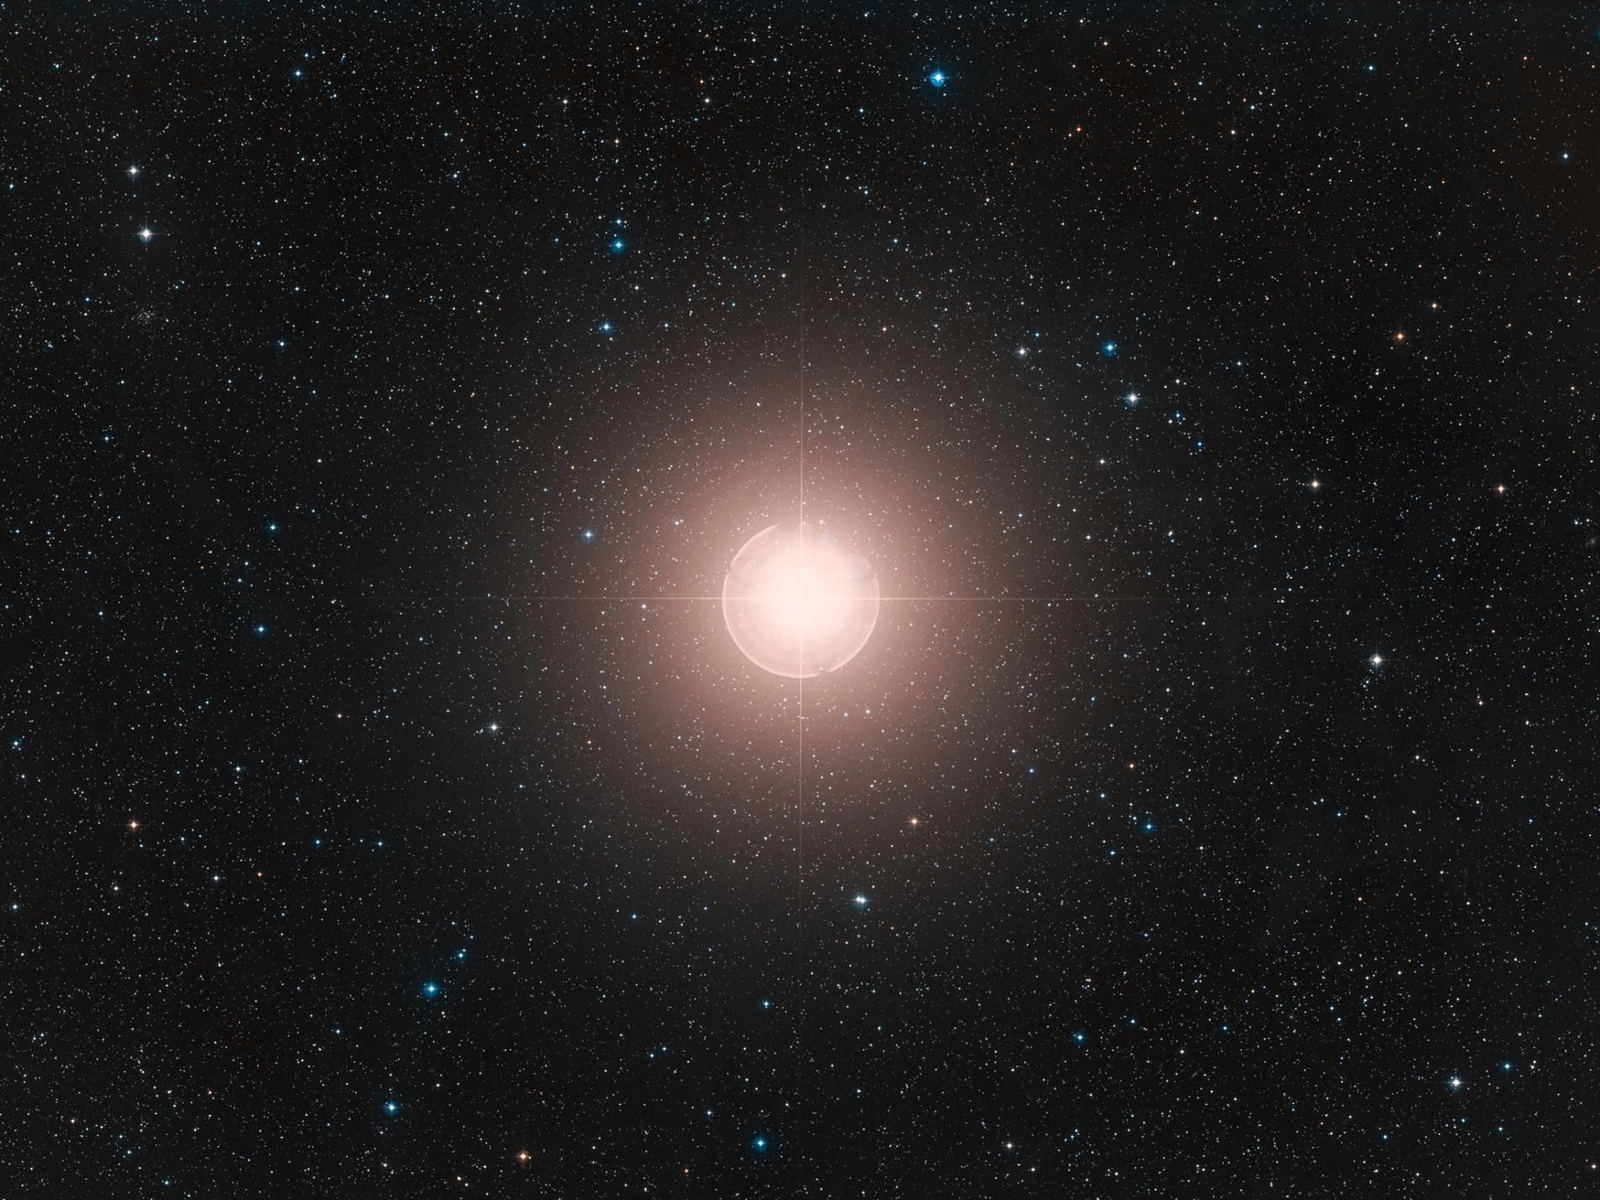
\includegraphics[%height=\paperheight,
      width=\paperwidth]{figure/etoile}}
  \begin{frame}[plain]
    \titlepage
  \end{frame}
}



%\section*{Executive Summary}

\begin{frame}{Executive Summary}
  \fontsize{8}{8}\selectfont
  \begin{block}{Context}
    Reliability Stress-Strength computations and Validation Plans are done with various methods \& tools within the group that are not always shared and not always up to date.
  \end{block}

  \begin{block}{Key points}
    \begin{itemize}
    \item Python module with easy-to-use notebook interface
    \item Full sphinx documentation
    \item Features
      \begin{itemize}
      \item (Non-)parametric distribution fitting using factories or kernel smoothing
      \item Taking into account extreme values for distribution tail fitting
      \item Stress projection
      \item Graphs for engineering judgment
      \end{itemize}
    \end{itemize}
  \end{block}

  % \begin{block}{Timeline}
  %     \begin{itemize}
  %         \item Reliability Stress-Strength computation tool with Python/OpenTURNS
  %         \item 2022 : Proof Of Concept achieved by INSA Rouen Intern
  %         \item 2023 : [Ex] StaRe : Renault Group specific python module with Phimeca
  %         \item 2024 : User interface integrated to platform ?
  %     \end{itemize}
  % \end{block}
\end{frame}

%-----------------------------------------
\begin{frame}{Table of Contents}
  \tableofcontents %[hideallsubsections]
\end{frame}

%-----------------------------

\section{Reliability pipeline and StaRe}
\begin{frame}{Reliability pipeline}
  \begin{center}
    \resizebox{.8\textwidth}{!}{
      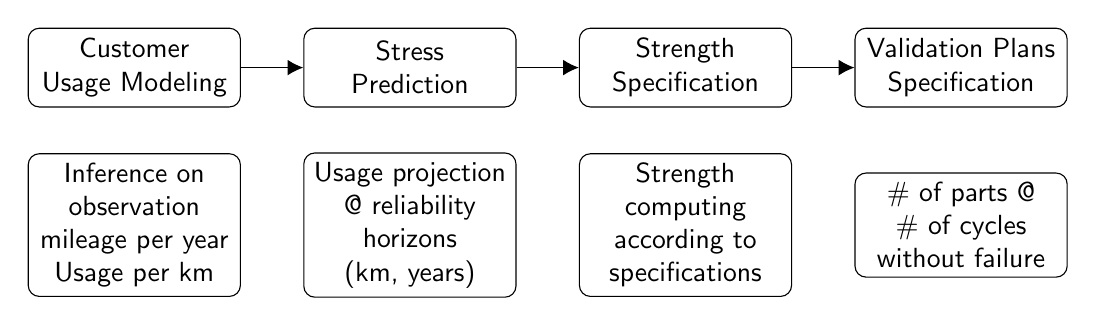
\begin{tikzpicture}[node distance=1.5cm,
          every node/.style={fill=white, font=\sffamily}, align=center]
        % Specification of nodes (position, etc.)
        \node(Go)[basebis]{Customer Usage Modeling};
        \node(Godesc)[basebis, below of=Go, yshift=-0.5cm]{Inference on observation mileage per year Usage per km};
        \node(Id)[basebis,right of=Go,xshift=2.cm]{
          Stress \\
          Prediction
        };
        \node(Iddesc)[basebis, below of=Id, yshift=-0.5cm]{Usage projection @ reliability horizons (km, years)};
        \node(MVP)[basebis,right of=Id,xshift=2.cm]{Strength \\ Specification};
        \node(MVPdesc)[basebis, below of=MVP, yshift=-0.5cm]{Strength computing according to specifications};
        \node(Indus)[basebis,right of=MVP,xshift=2.cm]{Validation Plans Specification};
        \node(Indusdesc)[basebis, below of=Indus, yshift=-0.5cm]{\# of parts @ \# of cycles without failure};
        \draw[->](Go) -- (Id);
        \draw[->](Id) -- (MVP);
        \draw[->](MVP) -- (Indus);
    \end{tikzpicture}}
  \end{center}
\end{frame}

\section{Customer data modelling}
\begin{frame}{StaRe : Customer Usage observation}
  \begin{center}
    \resizebox{.8\textwidth}{!}{
      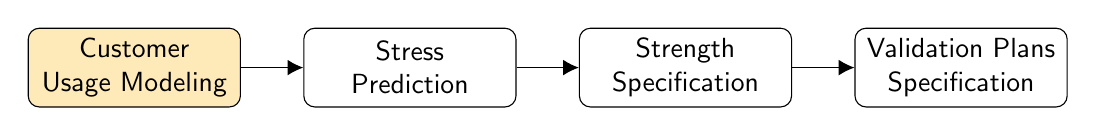
\begin{tikzpicture}[node distance=1.5cm,
          every node/.style={fill=white, font=\sffamily}, align=center]
        % Specification of nodes (position, etc.)
        \node(Go)[basebis,fill=color1!30]{Customer Usage Modeling};
        \node(Id)[basebis,right of=Go,xshift=2.cm]{
          Stress \\
          Prediction
        };
        \node(MVP)[basebis,right of=Id,xshift=2.cm]{Strength \\ Specification};
        \node(Indus)[basebis,right of=MVP,xshift=2.cm]{Validation Plans Specification};
        \draw[->](Go) -- (Id);
        \draw[->](Id) -- (MVP);
        \draw[->](MVP) -- (Indus);
    \end{tikzpicture}}
    \begin{columns}[t]
      \fontsize{8}{8}\selectfont
      \begin{column}{0.35\textwidth}
        \begin{itemize}
        \item Usage-Mileage scatter plot
        \end{itemize}
        \begin{figure}
          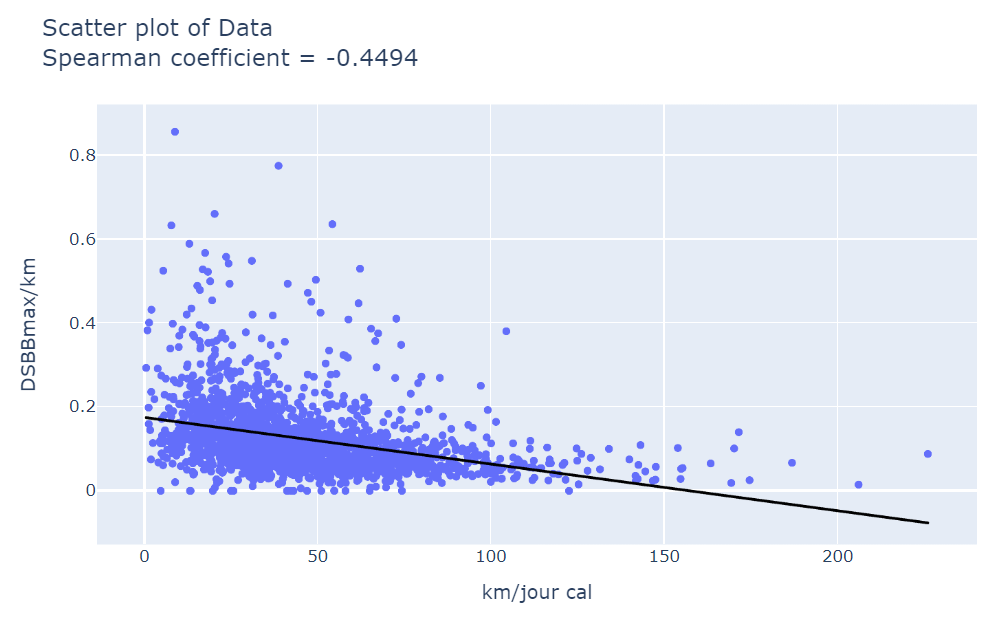
\includegraphics[height=0.44\textheight]{Illustration_StaRe/usageMileage.png}
        \end{figure}
      \end{column}

      \begin{column}{0.25\textwidth}
        \begin{itemize}
        \item Usage-Mileage scatter plot in rank space
        \end{itemize}
        \begin{figure}
          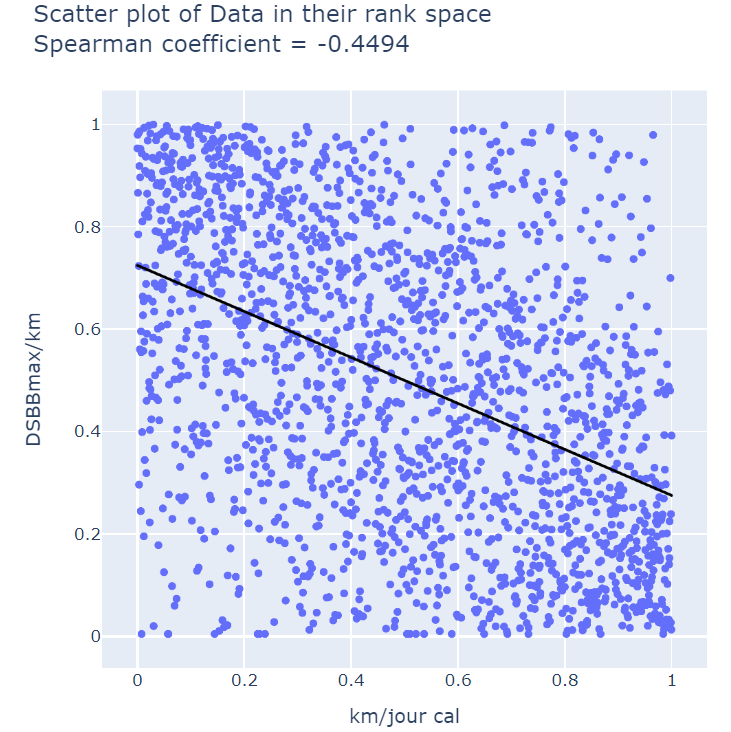
\includegraphics[height=0.44\textheight]{Illustration_StaRe/usageMileageRank.png}
        \end{figure}
      \end{column}

      \begin{column}{0.35\textwidth}
        \begin{itemize}
        \item Usage Mean Excess Plot for GDP threshold confirmation
        \end{itemize}
        \begin{figure}
          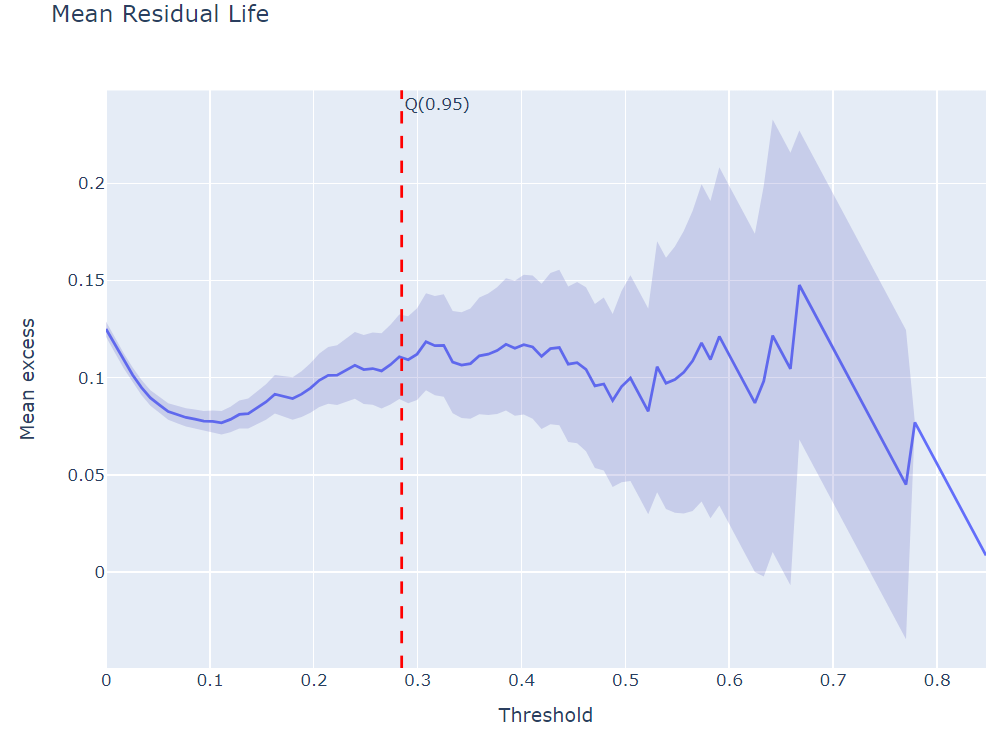
\includegraphics[height=0.44\textheight]{Illustration_StaRe/MRL.png}
        \end{figure}
      \end{column}
    \end{columns}
  \end{center}
\end{frame}

\begin{frame}{StaRe : Customer Usage observation}
  \begin{block}{Details}
    \begin{itemize}
    \item Raw data from csv imported as openturns.Sample/pandas.DataFrame
    \item Plotly visualization for enhanced interactivity
    \item As the module was developed with OTv1.21, Mean Excess Plot has been re-implemented
    \end{itemize}
  \end{block}
  \begin{figure}
    \centering
    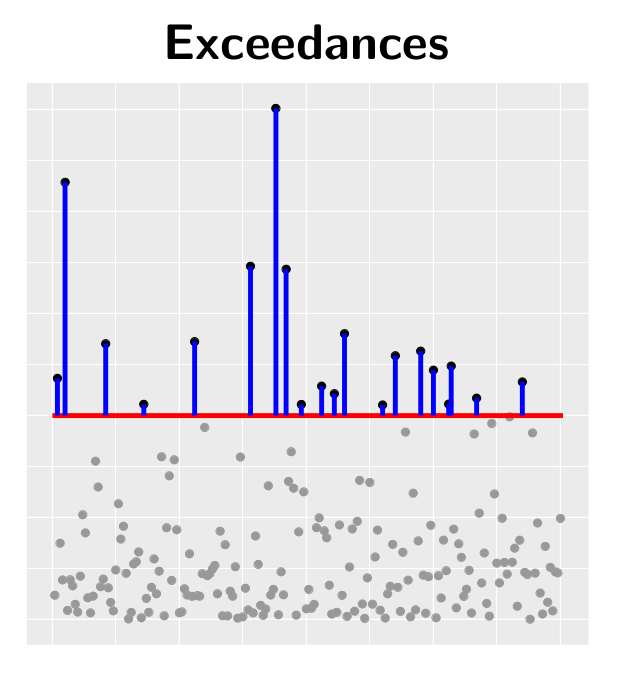
\includegraphics[height=0.44\textheight]{Illustration_StaRe/exceedances.png}
    \caption{from Thomas Opitz, atelier statistique de la SFdS.}
  \end{figure}
\end{frame}

\begin{frame}{StaRe : Customer Usage modelling}
  \begin{columns}[t]
    \fontsize{8}{8}\selectfont

    \begin{column}{0.5\textwidth}
      \begin{itemize}
      \item List of fitted distributions ordered by AIC or BIC or K score.
      \item Visual validation plots of the chosen distribution\\
        (here, Gumbel with GPD tail fit)
      \end{itemize}
      \begin{figure}
        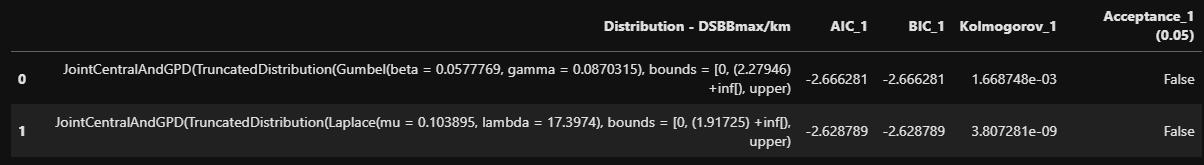
\includegraphics[width=\textwidth]{Illustration_StaRe/fit_results_table.png}
      \end{figure}
    \end{column}

    \begin{column}{0.5\textwidth}
      \begin{figure}
        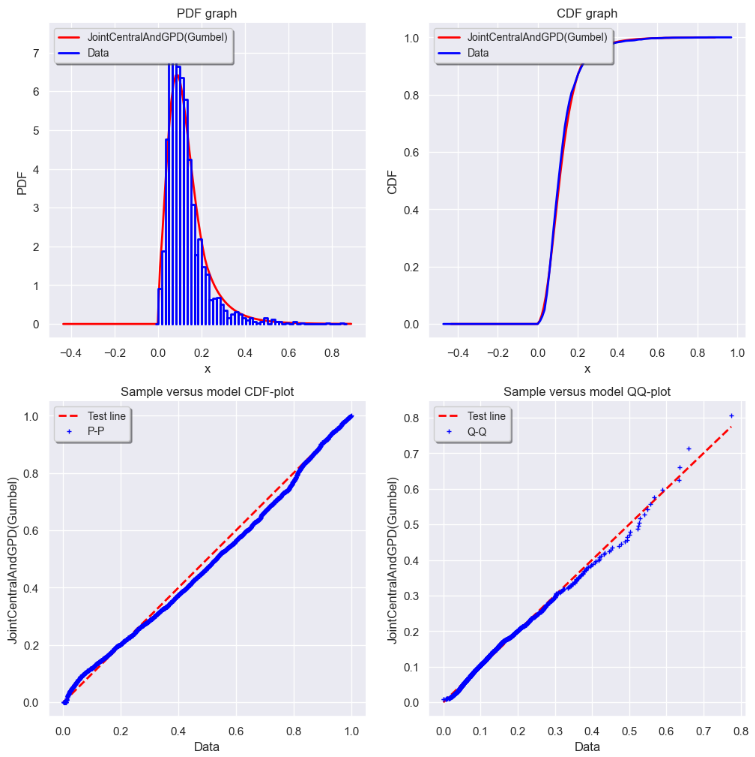
\includegraphics[width=0.8\textwidth]{Illustration_StaRe/fit_results.png}
      \end{figure}
    \end{column}
  \end{columns}

\end{frame}

\begin{frame}{StaRe : Mileage-Usage dependency fitting}
  \begin{columns}[t]
    \fontsize{8}{8}\selectfont

    \begin{column}{0.5\textwidth}
      \begin{itemize}
      \item Copula inference using all available copulae factories
      \end{itemize}
      \begin{figure}
        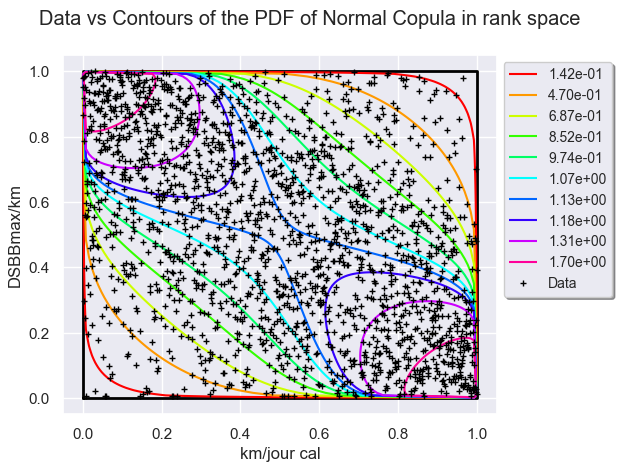
\includegraphics[width=0.5\textwidth]{Illustration_StaRe/fit_copula.png}
      \end{figure}
      \begin{figure}
        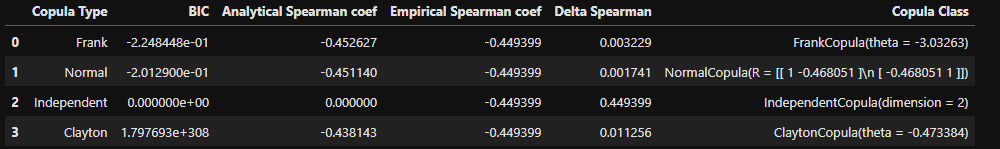
\includegraphics[width=\textwidth]{Illustration_StaRe/fit_copula_table.png}
      \end{figure}
    \end{column}

    \begin{column}{0.5\textwidth}
      \begin{itemize}
      \item JointDistribution built using marginal and copula inference results
      \end{itemize}
      \begin{figure}
        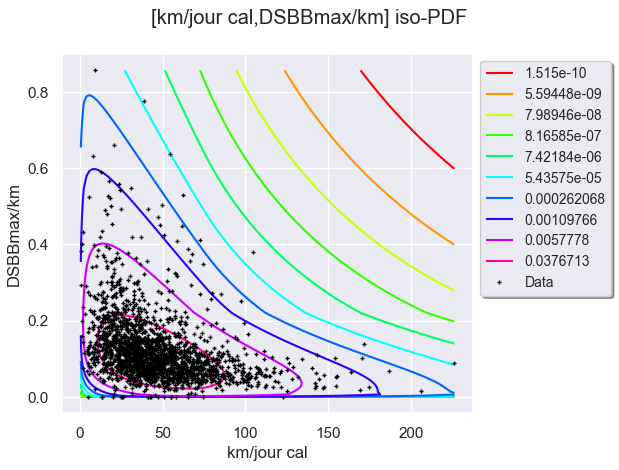
\includegraphics[width=0.8\textwidth]{Illustration_StaRe/joint_dist.png}
      \end{figure}
    \end{column}
  \end{columns}
\end{frame}

\begin{frame}{StaRe : Customer Usage modelling}
  \begin{block}{Details}
    \begin{itemize}
    \item Marginal inference handles truncated fit support\\
      Fit is performed using MaximumLikelihoodFactory, taking into account truncation parameters
    \item JointCentralAndGPD inherits from openturns.PythonDistribution\\
      computeCDF(), computePDF(), computeQuantile() and getRealization() have been re-implemented to ensure PDF continuity and to improve performance
    \end{itemize}
  \end{block}

  \begin{columns}[t]
    \begin{column}{0.4\textwidth}
      \begin{figure}
        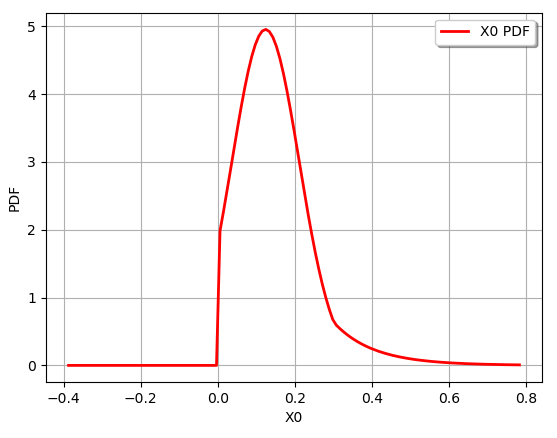
\includegraphics[width=0.45\textwidth]{Illustration_StaRe/PDF.png}
        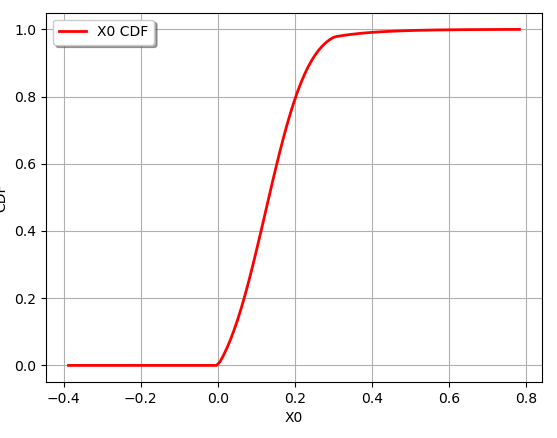
\includegraphics[width=0.45\textwidth]{Illustration_StaRe/CDF.png}
      \end{figure}
    \end{column}
    \begin{column}{0.6\textwidth}
      \small
      \[
      CDF(X) = \left\{
      \begin{array}{
          l@{}
          r@{}% no padding
        }
        CDF_{central}(X)                               &, \text{if }X \leq X_t \\
        1 - cCDF_{GPD}(X - X_t) \cdot cCDF_{central}(X_t)  &, \text{if } X \geq X_t \\
      \end{array}
      \right.
      \]
      \[
      PDF(X) = \left\{
      \begin{array}{
          l@{}
          r@{}% no padding
        }
        PDF_{central}(X)                                               &, \text{if } X \leq X_t \\
        PDF_{GPD}(X - X_t) \cdot \frac{PDF_{central}(X_t)}{PDF_{GPD}(0)}  &, \text{if } X \geq X_t\\
      \end{array}
      \right.
      \]

    \end{column}
  \end{columns}
\end{frame}

\section{Stress prediction}
\begin{frame}{Stress prediction : 2 algorithms}
  \begin{center}
    \resizebox{.8\textwidth}{!}{
      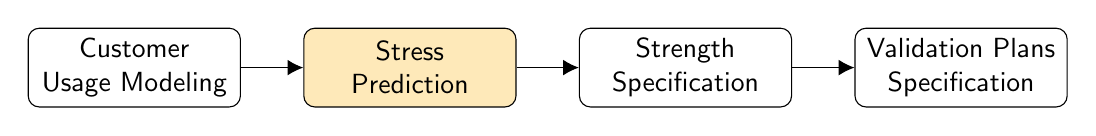
\begin{tikzpicture}[node distance=1.5cm,
          every node/.style={fill=white, font=\sffamily}, align=center]
        % Specification of nodes (position, etc.)
        \node(Go)[basebis]{Customer Usage Modeling};
        \node(Id)[basebis,fill=color1!30,right of=Go,xshift=2.cm]{
          Stress \\
          Prediction
        };
        \node(MVP)[basebis,right of=Id,xshift=2.cm]{Strength \\ Specification};
        \node(Indus)[basebis,right of=MVP,xshift=2.cm]{Validation Plans Specification};
        \draw[->](Go) -- (Id);
        \draw[->](Id) -- (MVP);
        \draw[->](MVP) -- (Indus);
    \end{tikzpicture}}
  \end{center}
  \begin{columns}[t]
    \fontsize{8}{8}\selectfont

    \begin{column}{0.4\textwidth}
      \begin{itemize}
      \item Historical algorithm
      \item Simulated car by simulated car
      \item Month by month
      \end{itemize}
    \end{column}

    \begin{column}{0.6\textwidth}
      \begin{figure}
        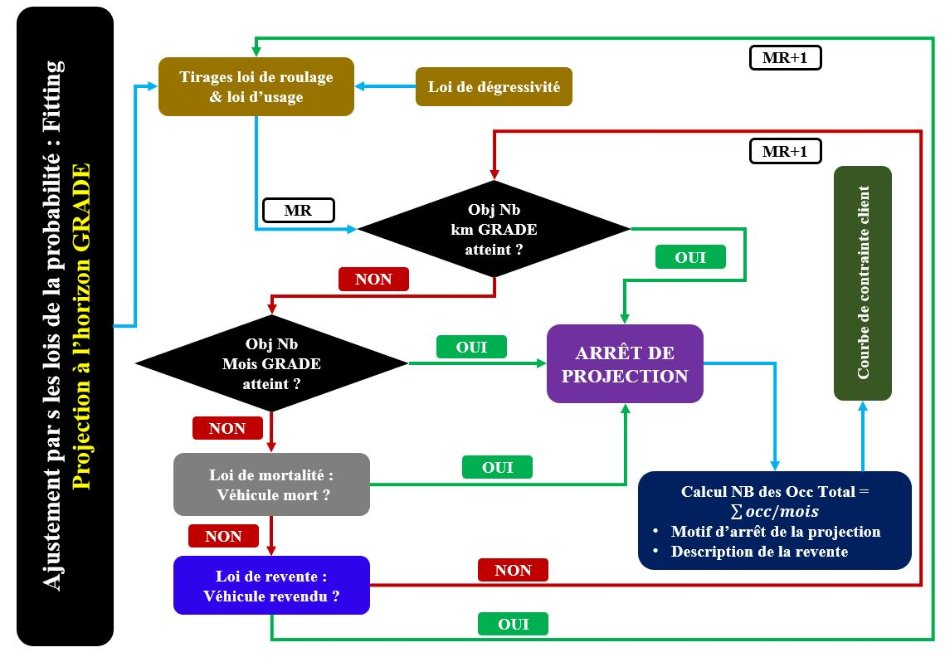
\includegraphics[width=0.8\textwidth]{Illustration_StaRe/algo_proj.png}
      \end{figure}
    \end{column}
  \end{columns}
\end{frame}

\begin{frame}{Stress prediction : 2 algorithms}
  \begin{center}
    \resizebox{.8\textwidth}{!}{
      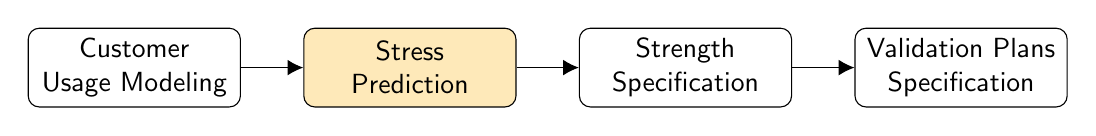
\begin{tikzpicture}[node distance=1.5cm,
          every node/.style={fill=white, font=\sffamily}, align=center]
        % Specification of nodes (position, etc.)
        \node(Go)[basebis]{Customer Usage Modeling};
        \node(Id)[basebis,fill=color1!30,right of=Go,xshift=2.cm]{
          Stress \\
          Prediction
        };
        \node(MVP)[basebis,right of=Id,xshift=2.cm]{Strength \\ Specification};
        \node(Indus)[basebis,right of=MVP,xshift=2.cm]{Validation Plans Specification};
        \draw[->](Go) -- (Id);
        \draw[->](Id) -- (MVP);
        \draw[->](MVP) -- (Indus);
    \end{tikzpicture}}
  \end{center}

  \begin{itemize}
  \item New algorithm, vector of simulated cars, car life event by car life event \\$\rightarrow$ Allows 200 times faster prediction
  \end{itemize}
  \begin{figure}
    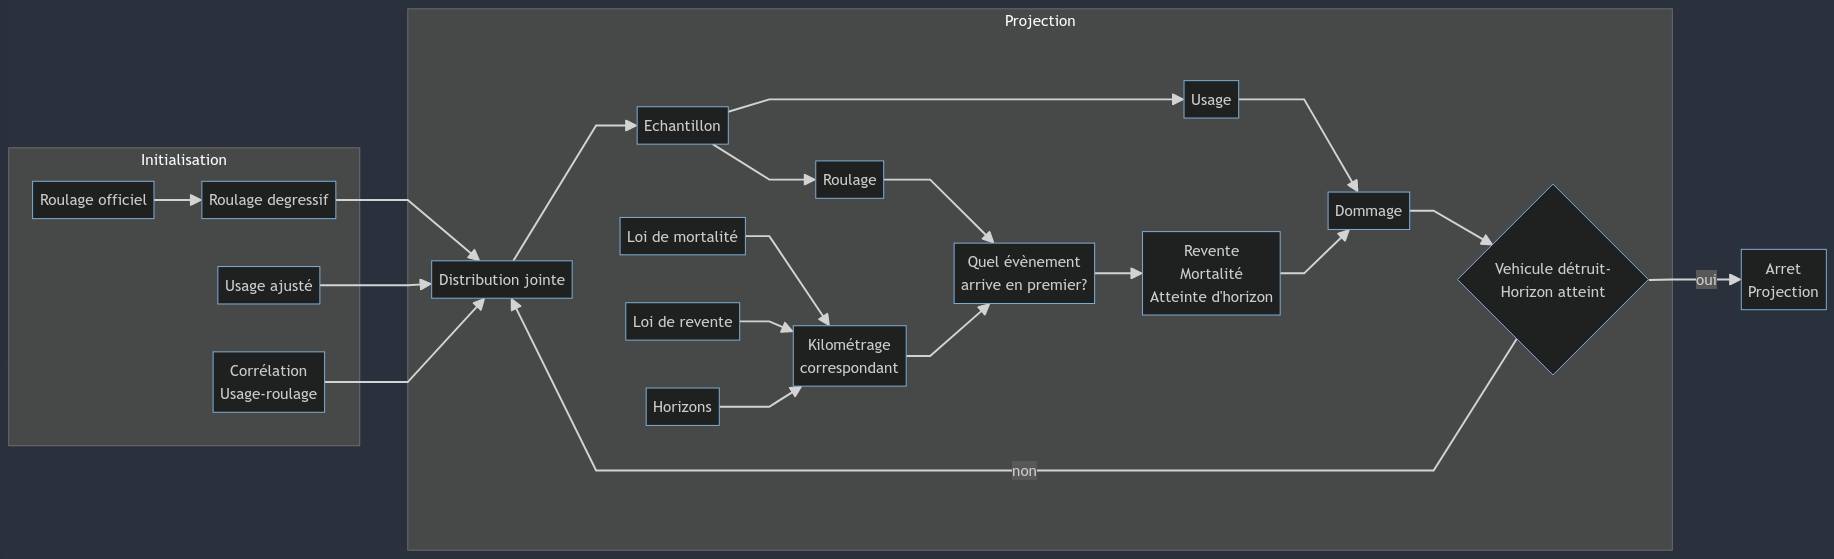
\includegraphics[width=\textwidth]{Illustration_StaRe/algo_proj2.png}
  \end{figure}
\end{frame}

\begin{frame}{Stress fitting}
  \begin{center}
    \resizebox{.8\textwidth}{!}{
      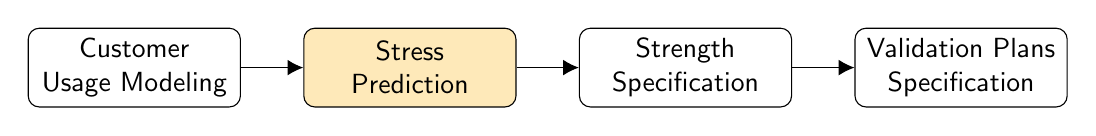
\begin{tikzpicture}[node distance=1.5cm,
          every node/.style={fill=white, font=\sffamily}, align=center]
        % Specification of nodes (position, etc.)
        \node(Go)[basebis]{Customer Usage Modeling};
        \node(Id)[basebis,fill=color1!30,right of=Go,xshift=2.cm]{
          Stress \\
          Prediction
        };
        \node(MVP)[basebis,right of=Id,xshift=2.cm]{Strength \\ Specification};
        \node(Indus)[basebis,right of=MVP,xshift=2.cm]{Validation Plans Specification};
        \draw[->](Go) -- (Id);
        \draw[->](Id) -- (MVP);
        \draw[->](MVP) -- (Indus);
    \end{tikzpicture}}
  \end{center}
  \begin{itemize}
  \item Stress prediction distribution is fitted using the same methods applied previously to raw data
  \end{itemize}
  \begin{figure}
    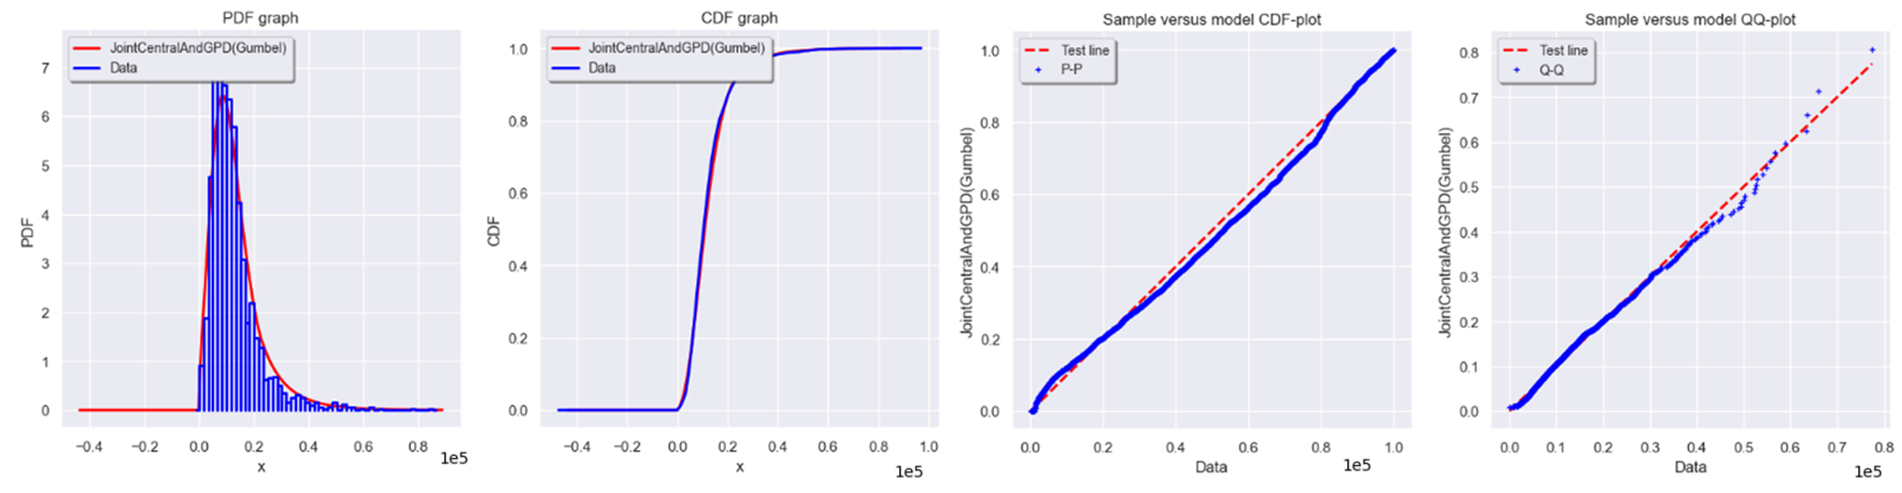
\includegraphics[width=\textwidth]{Illustration_StaRe/fitted_c.png}
  \end{figure}
\end{frame}

\section{Strength specification}
\begin{frame}{Strength specification}
  \begin{center}
    \resizebox{.8\textwidth}{!}{
      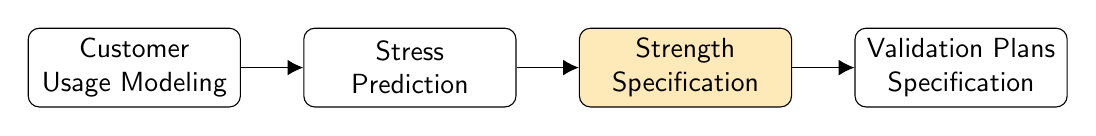
\begin{tikzpicture}[node distance=1.5cm,
          every node/.style={fill=white, font=\sffamily}, align=center]
        % Specification of nodes (position, etc.)
        \node(Go)[basebis]{Customer Usage Modeling};
        \node(Id)[basebis,right of=Go,xshift=2.cm]{
          Stress \\
          Prediction
        };
        \node(MVP)[basebis,fill=color1!30,right of=Id,xshift=2.cm]{Strength \\ Specification};
        \node(Indus)[basebis,right of=MVP,xshift=2.cm]{Validation Plans Specification};
        \draw[->](Go) -- (Id);
        \draw[->](Id) -- (MVP);
        \draw[->](MVP) -- (Indus);
    \end{tikzpicture}}
  \end{center}
  \begin{columns}
    \begin{column}{0.4\textwidth}
      \begin{itemize}
      \item With hypothesis on shape parameter, strength scale parameter is optimized to match \\ proba (Stress > Strength) max
      \item Strength is modelised by LogNormal or WeibullMin distribution
      \item Stress 99$^{th}$ percentile $\sim 8.4 \cdot 10^4$ in this case
      \end{itemize}
    \end{column}
    \begin{column}{0.6\textwidth}
      \begin{figure}
        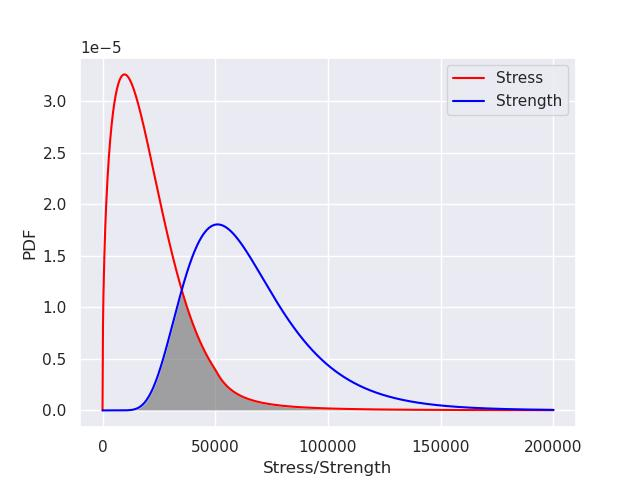
\includegraphics[width=0.80\textwidth]{Illustration_StaRe/CR11.0.jpg}
      \end{figure}
    \end{column}
  \end{columns}
\end{frame}

\begin{frame}{Strength specification}
  \begin{center}
    \resizebox{.8\textwidth}{!}{
      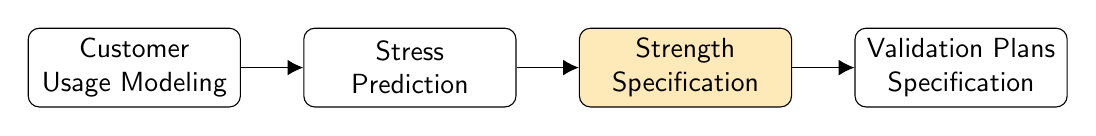
\begin{tikzpicture}[node distance=1.5cm,
          every node/.style={fill=white, font=\sffamily}, align=center]
        % Specification of nodes (position, etc.)
        \node(Go)[basebis]{Customer Usage Modeling};
        \node(Id)[basebis,right of=Go,xshift=2.cm]{
          Stress \\
          Prediction
        };
        \node(MVP)[basebis,fill=color1!30,right of=Id,xshift=2.cm]{Strength \\ Specification};
        \node(Indus)[basebis,right of=MVP,xshift=2.cm]{Validation Plans Specification};
        \draw[->](Go) -- (Id);
        \draw[->](Id) -- (MVP);
        \draw[->](MVP) -- (Indus);
    \end{tikzpicture}}
  \end{center}
  \begin{columns}
    \begin{column}{0.4\textwidth}
      \begin{itemize}
      \item With hypothesis on shape parameter, strength scale parameter is optimized to match \\ proba (Stress > Strength) max
      \item Strength is modelised by LogNormal or WeibullMin distribution
      \item Stress 99$^{th}$ percentile $\sim 8.4 \cdot 10^4$ in this case
      \end{itemize}
    \end{column}
    \begin{column}{0.6\textwidth}
      \begin{figure}
        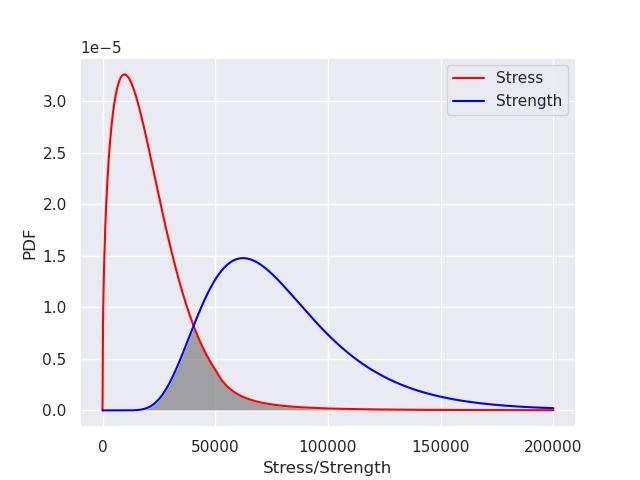
\includegraphics[width=0.80\textwidth]{Illustration_StaRe/CR11.2.jpg}
      \end{figure}
    \end{column}
  \end{columns}
\end{frame}

\begin{frame}{Strength specification}
  \begin{center}
    \resizebox{.8\textwidth}{!}{
      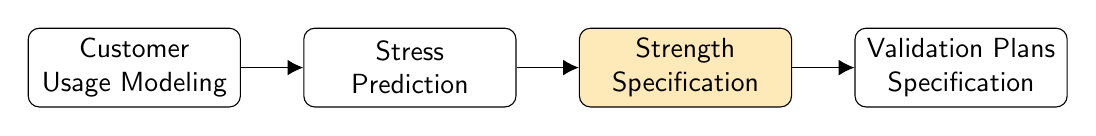
\begin{tikzpicture}[node distance=1.5cm,
          every node/.style={fill=white, font=\sffamily}, align=center]
        % Specification of nodes (position, etc.)
        \node(Go)[basebis]{Customer Usage Modeling};
        \node(Id)[basebis,right of=Go,xshift=2.cm]{
          Stress \\
          Prediction
        };
        \node(MVP)[basebis,fill=color1!30,right of=Id,xshift=2.cm]{Strength \\ Specification};
        \node(Indus)[basebis,right of=MVP,xshift=2.cm]{Validation Plans Specification};
        \draw[->](Go) -- (Id);
        \draw[->](Id) -- (MVP);
        \draw[->](MVP) -- (Indus);
    \end{tikzpicture}}
  \end{center}
  \begin{columns}
    \begin{column}{0.4\textwidth}
      \begin{itemize}
      \item With hypothesis on shape parameter, strength scale parameter is optimized to match \\ proba (Stress > Strength) max
      \item Strength is modelised by LogNormal or WeibullMin distribution
      \item Stress 99$^{th}$ percentile $\sim 8.4 \cdot 10^4$ in this case
      \end{itemize}
    \end{column}
    \begin{column}{0.6\textwidth}
      \begin{figure}
        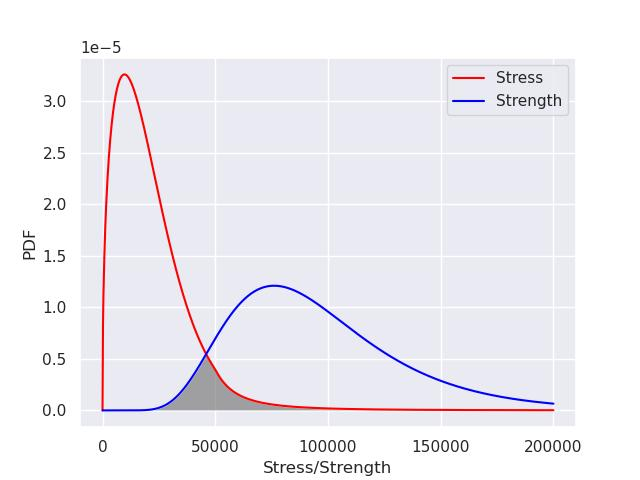
\includegraphics[width=0.80\textwidth]{Illustration_StaRe/CR11.4.jpg}
      \end{figure}
    \end{column}
  \end{columns}
\end{frame}

\begin{frame}{Strength specification}
  \begin{center}
    \resizebox{.8\textwidth}{!}{
      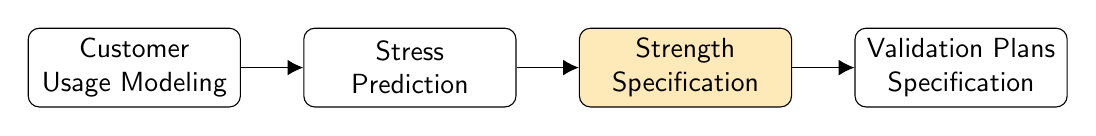
\begin{tikzpicture}[node distance=1.5cm,
          every node/.style={fill=white, font=\sffamily}, align=center]
        % Specification of nodes (position, etc.)
        \node(Go)[basebis]{Customer Usage Modeling};
        \node(Id)[basebis,right of=Go,xshift=2.cm]{
          Stress \\
          Prediction
        };
        \node(MVP)[basebis,fill=color1!30,right of=Id,xshift=2.cm]{Strength \\ Specification};
        \node(Indus)[basebis,right of=MVP,xshift=2.cm]{Validation Plans Specification};
        \draw[->](Go) -- (Id);
        \draw[->](Id) -- (MVP);
        \draw[->](MVP) -- (Indus);
    \end{tikzpicture}}
  \end{center}
  \begin{columns}
    \begin{column}{0.4\textwidth}
      \begin{itemize}
      \item With hypothesis on shape parameter, strength scale parameter is optimized to match \\ proba (Stress > Strength) max
      \item Strength is modelised by LogNormal or WeibullMin distribution
      \item Stress 99$^{th}$ percentile $\sim 8.4 \cdot 10^4$ in this case
      \end{itemize}
    \end{column}
    \begin{column}{0.6\textwidth}
      \begin{figure}
        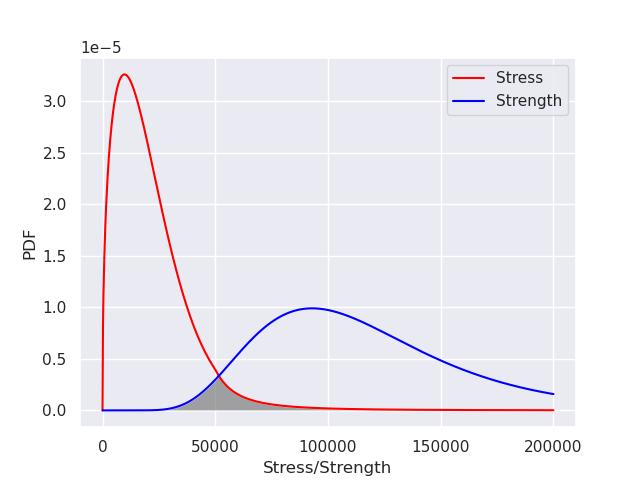
\includegraphics[width=0.80\textwidth]{Illustration_StaRe/CR11.6.jpg}
      \end{figure}
    \end{column}
  \end{columns}
\end{frame}

\begin{frame}{Strength specification}
  \begin{center}
    \resizebox{.8\textwidth}{!}{
      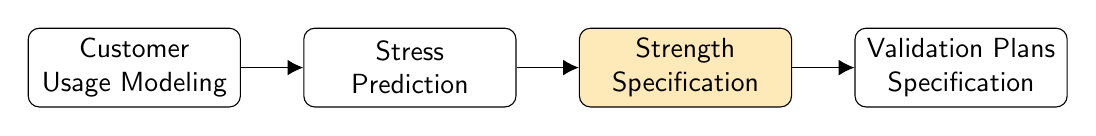
\begin{tikzpicture}[node distance=1.5cm,
          every node/.style={fill=white, font=\sffamily}, align=center]
        % Specification of nodes (position, etc.)
        \node(Go)[basebis]{Customer Usage Modeling};
        \node(Id)[basebis,right of=Go,xshift=2.cm]{
          Stress \\
          Prediction
        };
        \node(MVP)[basebis,fill=color1!30,right of=Id,xshift=2.cm]{Strength \\ Specification};
        \node(Indus)[basebis,right of=MVP,xshift=2.cm]{Validation Plans Specification};
        \draw[->](Go) -- (Id);
        \draw[->](Id) -- (MVP);
        \draw[->](MVP) -- (Indus);
    \end{tikzpicture}}
  \end{center}
  \begin{columns}
    \begin{column}{0.4\textwidth}
      \begin{itemize}
      \item With hypothesis on shape parameter, strength scale parameter is optimized to match \\ proba (Stress > Strength) max
      \item Strength is modelised by LogNormal or WeibullMin distribution
      \item Stress 99$^{th}$ percentile $\sim 8.4 \cdot 10^4$ in this case
      \end{itemize}
    \end{column}
    \begin{column}{0.6\textwidth}
      \begin{figure}
        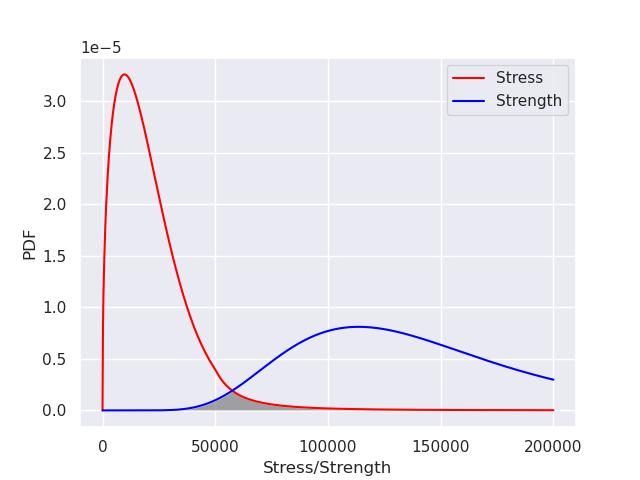
\includegraphics[width=0.80\textwidth]{Illustration_StaRe/CR11.8.jpg}
      \end{figure}
    \end{column}
  \end{columns}
\end{frame}

\section{Validation plan specification}
\begin{frame}{Validation plan specification}
  \begin{center}
    \resizebox{.8\textwidth}{!}{
      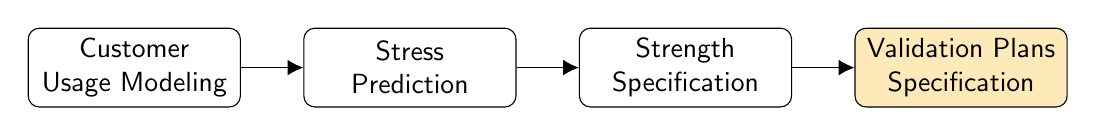
\begin{tikzpicture}[node distance=1.5cm,
          every node/.style={fill=white, font=\sffamily}, align=center]
        % Specification of nodes (position, etc.)
        \node(Go)[basebis]{Customer Usage Modeling};
        \node(Id)[basebis,right of=Go,xshift=2.cm]{
          Stress \\
          Prediction
        };
        \node(MVP)[basebis,right of=Id,xshift=2.cm]{Strength \\ Specification};
        \node(Indus)[basebis,fill=color1!30,right of=MVP,xshift=2.cm]{Validation Plans Specification};
        \draw[->](Go) -- (Id);
        \draw[->](Id) -- (MVP);
        \draw[->](MVP) -- (Indus);
    \end{tikzpicture}}
  \end{center}
  \begin{columns}[t]
    \fontsize{8}{8}\selectfont

    \begin{column}{0.6\textwidth}
      \begin{itemize}
      \item Validation plan proposal : \\
        Number of parts @ number of cycles without failure
      \item Strength is tested by statistical hypothesis with confidence level:\\
        Hypothesis on proportion of failures is tested (unilateral) on small sample without failure \\
        $\rightarrow$ binomial distribution with number of success (ie failure) equal to 0
      \end{itemize}
    \end{column}
    \begin{column}{0.4\textwidth}
      \begin{figure}
        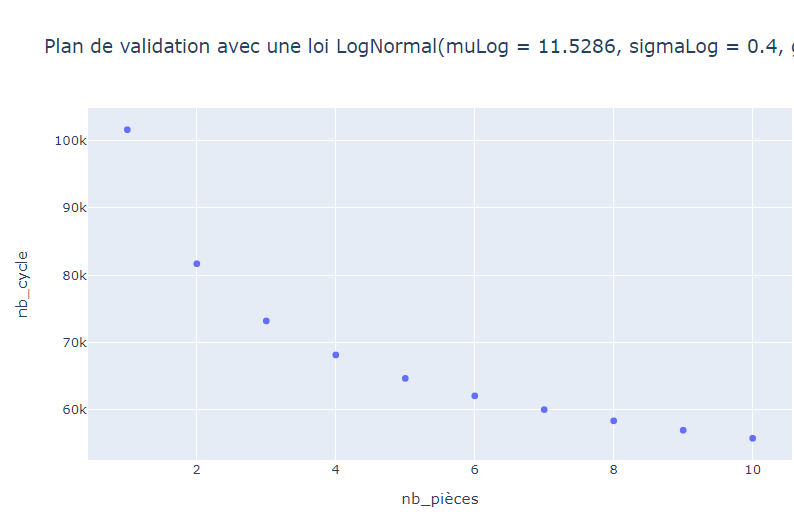
\includegraphics[width=\textwidth]{Illustration_StaRe/validation_plan.png}
      \end{figure}
    \end{column}
  \end{columns}
\end{frame}

\begin{frame}{Validation plan specification}
  \begin{center}
    \resizebox{.8\textwidth}{!}{
      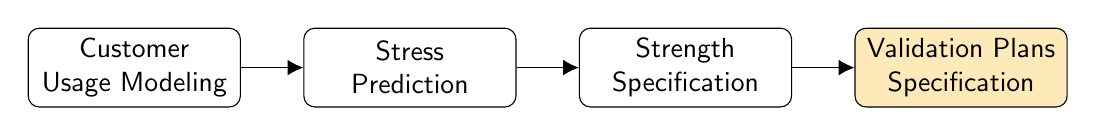
\begin{tikzpicture}[node distance=1.5cm,
          every node/.style={fill=white, font=\sffamily}, align=center]
        % Specification of nodes (position, etc.)
        \node(Go)[basebis]{Customer Usage Modeling};
        \node(Id)[basebis,right of=Go,xshift=2.cm]{
          Stress \\
          Prediction
        };
        \node(MVP)[basebis,right of=Id,xshift=2.cm]{Strength \\ Specification};
        \node(Indus)[basebis,fill=color1!30,right of=MVP,xshift=2.cm]{Validation Plans Specification};
        \draw[->](Go) -- (Id);
        \draw[->](Id) -- (MVP);
        \draw[->](MVP) -- (Indus);
    \end{tikzpicture}}
  \end{center}

  \begin{columns}[t]
    \fontsize{8}{8}\selectfont

    \begin{column}{0.6\textwidth}
      \begin{itemize}
      \item Reciprocal procedure available : \\
        From a number of parts, each with number of cycles with (and/or without) failure
      \item Strength distribution scale parameter is determined leading to failure probability estimation
      \end{itemize}
    \end{column}
    \begin{column}{0.4\textwidth}
      \begin{figure}
        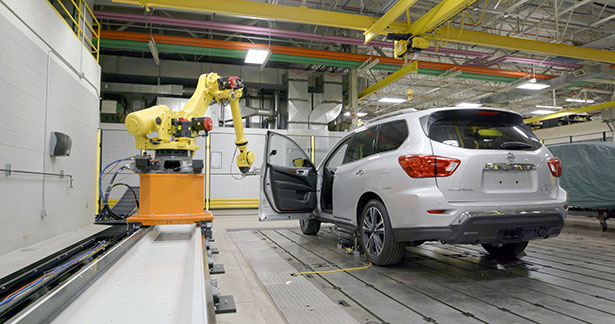
\includegraphics[width=\textwidth]{Illustration_StaRe/door-slamming-robot-blog-image.jpg}
      \end{figure}
    \end{column}
  \end{columns}
\end{frame}


\section*{Conclusion \& outlook}
\begin{frame}{Conclusion \& outlook}

  \begin{block}{Deployment: sharing good practices and methodology}
    \small
    \begin{center}
      \begin{tabular}{|c|c|c|c|c|c|}
        \hline
        Reliability&Python &Tool&Status&Trained&Interested\\
        & User  &    &      &       & \\
        \hline\hline
        Specialist & Yes & Stare module & Delivered&7&5\\
        &  & Notebook &  & & \\
        \hline
        Specialist&No&No code&Decided&0&10\\
        & &GUI& & & \\\hline
        Intermediate&No&Simple GUI&To be decided \& framed& & \\
        \hline
      \end{tabular}
    \end{center}
  \end{block}

  \begin{block}{Conclusion}
    \begin{itemize}
    \item StaRe module allows better distribution fitting leading to improved validation plans
    \item Dedicated notebook interface allows versatile reliability tools usage for (non-)coding experts
    \item Opening discussion for including in OT
      \begin{itemize}
      \item fit automatisation, taking into account support
      \item stare.JointCentralAndGPD implementation
      \end{itemize}
    \end{itemize}
  \end{block}

\end{frame}

\section*{Thank you!}
%\begin{frame}
%
\includegraphics[width=\textwidth]{figure/grpe_rno_black.png}
%\end{frame}

\end{document}
